\chapter{Background}
\section{Graphen}
Ein Graph repräsentiert eine Gruppe von Objekten und deren Verbindungen miteinander. Die einzelnen Objekte nennt man Knoten, während die Verbindungen als Kanten bezeichnet werden. Wie in Abbildung \ref{abb:graph} werden Knoten oft als Kreise dargestellt und Kanten als Linien, die zwei der Kreise miteinander verbinden. Graphen können verwendet werden um beispielsweise Netzwerke von Computern zu modellieren. In der Abbildung stünde dann jeder Kreis für einen Rechner im Netzwerk und jede Linie für eine Netzwerkverbindung. Es ist allerdings nicht nur möglich physische Objekte und Verbindungen darzustellen, sondern auch abstraktere Konzepte. Satzstrukturen in einem Buch könnten beispielsweise mit einem Graphen analysiert werden, indem jeder Knoten ein Wort aus dem Text darstellt und jede Kante anzeigt, dass zwei Wörter häufig zusammen in einem Satz auftauchen. Ein bekanntes Beispiel für den Praxiseinsatz von Graphen ist der $PageRank-Algorithmus$ \cite{page1999pagerank}, welcher als Basis für die Suchmaschine Google diente.

\subsection{Bäume}\label{sec:baum}
\begin{figure}
	\centering
	\begin{minipage}{.5\textwidth}
		\centering
		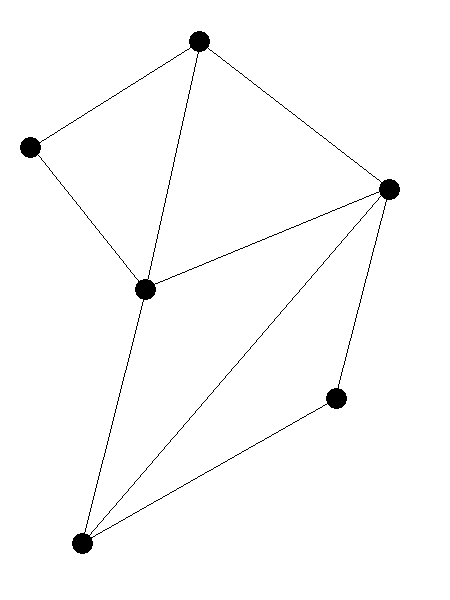
\includegraphics[width=.9\linewidth]{../screenshots/graphexample.PNG}
		\caption{Ein Beispiel für einen Graphen}
		\label{abb:graph}
	\end{minipage}%
	\begin{minipage}{.5\textwidth}
		\centering
		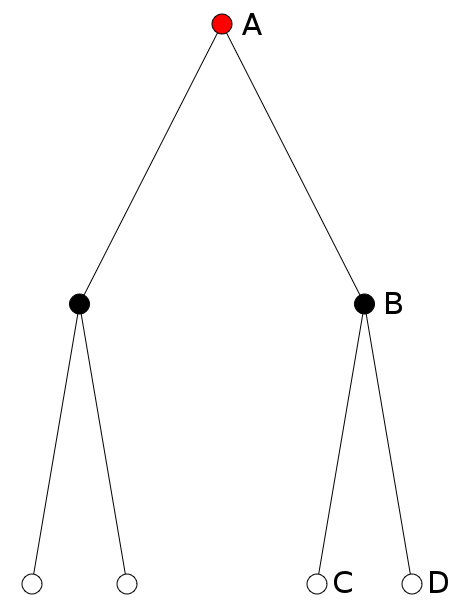
\includegraphics[width=.9\linewidth]{../screenshots/tree-example.PNG}
		\caption{Ein Beispiel für einen Baum}
		\label{abb:baum}
	\end{minipage}
\end{figure}
Die in dieser Arbeit beschriebene Visualisierung befasst sich mit Bäumen, welche eine spezielle Form von Graphen sind, für die zusätzliche Regeln gelten. Verbundene Knoten in einem Baum stehen in einer Vorgänger-Nachfolger Beziehung. Nachfolger eines Knotens werden auch als dessen Kinder bezeichnet. Zur Veranschaulichung ist auf Abbildung \ref{abb:baum} ein Baum dargestellt. Auf dem Bild ist $A$ der Vorgänger von Knoten $B$ und dessen Nachfolger sind $C$ und $D$. In einem Baum hat jeder Knoten genau einen Vorgänger und beliebig viele Nachfolger. Die einzige Ausnahme zu dieser Regel bildet die sogenannte Wurzel, die keinen Vorgänger hat und somit quasi der Ursprung des Baumes ist. In diesem Fall ist die Wurzel der rot dargestellte Knoten $A$. Von Blättern - hier in weiß dargestellt - spricht man, wenn Knoten keine Nachfolger haben. $B$ hat sowohl einen Vorgänger als auch Kinder, was ihn zu einem der inneren Knoten macht, die in schwarz abgebildet sind. Genauer gesagt sind alle Knoten, die keine Blätter sind, innere Knoten, was auch die Wurzel mit einschließt. Die Höhe eines Baumes bezeichnet die Strecke von der Wurzel bis zu dem Blatt, welches am weitesten entfernt ist. Die Entfernung misst man in der Anzahl an Knoten, die zwischen den Beiden liegen, wobei man die Wurzel und das Blatt mitzählt. In Abbildung \ref{abb:baum} wäre die Distanz von Knoten $A$ zu $D$ also 3. Das ist auch die Höhe des Baumes, da es kein Blatt gibt, das weiter von $A$ entfernt ist.

Bäume finden Anwendung in den verschiedensten Gebieten. Im Bereich der Künstlichen Intelligenz werden sie zur Ermittlung optimaler Züge in Brettspielen wie Schach verwendet, in der Ahnenforschung kennt man sie als Stammbäume und sie können zur Modellierung von Entscheidungsabfolgen genutzt werden. Im zuletzt genannten Fall spricht man auch von Entscheidungsbäumen.

\subsection{Entscheidungsbäume}
\begin{figure}
	\centering
	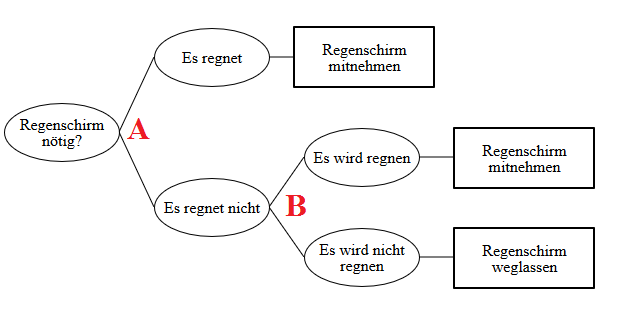
\includegraphics[width=.8\linewidth]{../screenshots/entscheidungsbaum_bsp.PNG}
	\caption{Ein simpler Entscheidungsbaum}
	\label{abb:entsch_baum_bsp}
\end{figure}
In Abbildung \ref{abb:entsch_baum_bsp} ist beispielhaft ein Entscheidungsbaum zu sehen, der in stark vereinfachter Form die Entscheidungsfindung zur Frage zeigt, ob beim Verlassen des Hauses ein Regenschirm mitgenommen werden sollte. Innere Knoten sind als Ellipsen dargestellt und Blätter, welche endgültige Ergebnisse repräsentieren, sind rechteckig. Die Beschriftung der Knoten zeigt an, welche Aussage oder Frage sie symbolisieren. Bei Verzweigung $A$ muss zwischen den Möglichkeiten \glqq Es regnet\grqq\ und \glqq Es regnet nicht\grqq\ entschieden werden, wobei im Ersten Fall sofort das Ergebnis \glqq Regenschirm mitnehmen\grqq\ erreicht wird. Regnet es nicht, so muss bei Verzweigung $B$ der Wetterbericht oder das Bauchgefühl zurate gezogen werden um zwischen den Möglichkeiten \glqq Es wird regnen\grqq\ und \glqq Es wird nicht regnen\grqq\ zu entscheiden, welche dann zu den Ergebnissen \glqq Regenschirm mitnehmen\grqq\ beziehungsweise \glqq Regenschirm weglassen\grqq\ führen.

Natürlich handelt es sich hierbei zum erleichterten Verständnis um ein sehr simples Beispiel. Man kann sich vorstellen, das bei der Repräsentation von komplexeren Abläufen, wie dem Behandlungsverfahren von Krankheiten bedeutend größere Bäume entstehen.

\section{SVG}\label{sec:svg}
SVG steht für \glqq Scalable Vector Graphics\grqq\ (kurz: Vektorgrafik) und bezeichnet eine vom World Wide Web Consortium aufgestellte Spezifikation zur Definition von Vektorgrafiken. \todo{quelle} Durch Verwendung des HTML-Elements $svg$ bietet sich damit eine einfache, von allen Browsern unterstützte Möglichkeit, Grafiken mit beliebigen Formen und Farben in eine Internetseite einzubinden. Dazu können im Inneren eines $svg$ verschiedene Elemente benutzt werden. Im Folgenden bezieht sich die Schreibweise \glqq SVG\grqq\ immer auf Vektorgrafiken im Allgemeinen, während mit $svg$ das HTML-Element gemeint ist.

\subsection{Geometrische Grundformen}
Für einige Grundformen gibt es eigene Elemente. Zum Beispiel kann mit $circle$ ein Kreis erzeugt werden, mit $rect$ ein Rechteck. Dabei können genaue Angaben über Position, Größe, Farbe, Umrandung und einige Andere Eigenschaften gemacht werden.

\subsection{Text}
Ein $text$-Element dient zur Anzeige von Schrift. Es kann entweder reinen Text enthalten, oder Unter-Elemente wie $tspan$. Sowohl beim $text$- als auch beim $tspan$-Element können beispielsweise Position, Farbe und Schriftgröße bestimmt werden. Die $tspan$-Elemente dienen dazu, diese Angaben nur für den in ihnen enthaltenen Teil des Textes zu machen. So kann ein Text zum Beispiel in mehrere Zeilen aufgeteilt werden, indem jede Zeile innerhalb eines $tspan$ steht und deren Positionierung entsprechend angepasst wird, was bei der Berechnung von Zeilenumbrüchen in Kapitel \ref{sec:zeilenumbrueche} zum Einsatz kommt.

\subsection{Path}
Zur Erzeugung komplexerer Formen dienen $path$-Elemente, die Pfade innerhalb des $svg$ beschreiben. Ein Pfad ist zunächst eine Linie mit beliebig vielen Ecken und Wendungen. Der Pfad, den die Linie beschreibt wird von der Eigenschaft $d$ festgelegt, welche eine Abfolge von Zeichenbefehlen enthält. Diese Liste von Anweisungen kann mit steigender Komplexität des Pfades sehr lang werden, weshalb das in Kapitel \ref{sec:framework} beschriebene D3 einige Funktionen zu deren Generierung anbietet. Auch bei Pfaden gilt wieder, dass ihr Aussehen was zum Beispiel Farbe angeht frei wählbar ist. Ist ein Pfad geschlossen, das heißt endet er dort wo er begonnen hat, dann kann auch eine Füllfarbe angegeben werden, mit der die vom Pfad eingeschlossene Fläche gefüllt wird.

\subsection{Gruppieren von Elementen}
Manchmal ist es wünschenswert zusammengehörende Elemente in Gruppen zusammenzufassen. Zu diesem Zweck gibt es $g$-Elemente, welche das Attribut $transform$ besitzen und beliebige andere Objekte, wie die zuvor beschriebenen $path$-, $circle$- oder $text$-Elemente enthalten können. Das $transform$-Attribut beschreibt Veränderungen, die an allen im $g$ enthaltenen Elementen vorgenommen werden. Erlaubte Transformationen sind  Verschiebung ($translate$), Skalierung ($scale$), Rotation ($rotation$) und Verzerrung ($skewX$ bzw. $skewY$). Verschiebt man auf diese Weise alle gruppierten Elemente, bleibt deren relative Positionierung zueinander erhalten, das heißt ein Text, der vor der Verschiebung in der Gruppe zentriert ist, bleibt das auch nach der Verschiebung.

SVG können eingesetzt werden um Statistiken und andere Daten zu visualisieren. Zur Vereinfachung dieser Aufgabe liefert die Javascript Bibliothek D3 zahlreiche Hilfsmittel.

\section{D3}\label{sec:framework}
D3 - kurz für Data-Driven Documents - ist eine unter BSD-Lizenz veröffentlichte Open-Source Javascript Bibliothek zur Visualisierung von Daten auf Internetseiten. Sie ist ein maßgebliches Hilfsmittel im Zuge dieser Arbeit. Das Konzept von D3 ist es, Datensätze mit Elementen eines HTML-Dokuments, wie $svg$ und dessen Unterelemente, zu verknüpfen und dadurch großen Einfluss auf die Darstellung dieser Daten zu haben. Dabei werden neben Hilfsfunktionen zum Strukturieren der Datenanzeige auch diverse Möglichkeiten zur Erstellung und Manipulierung von Datenstrukturen angeboten. 
\begin{figure}
	\centering
	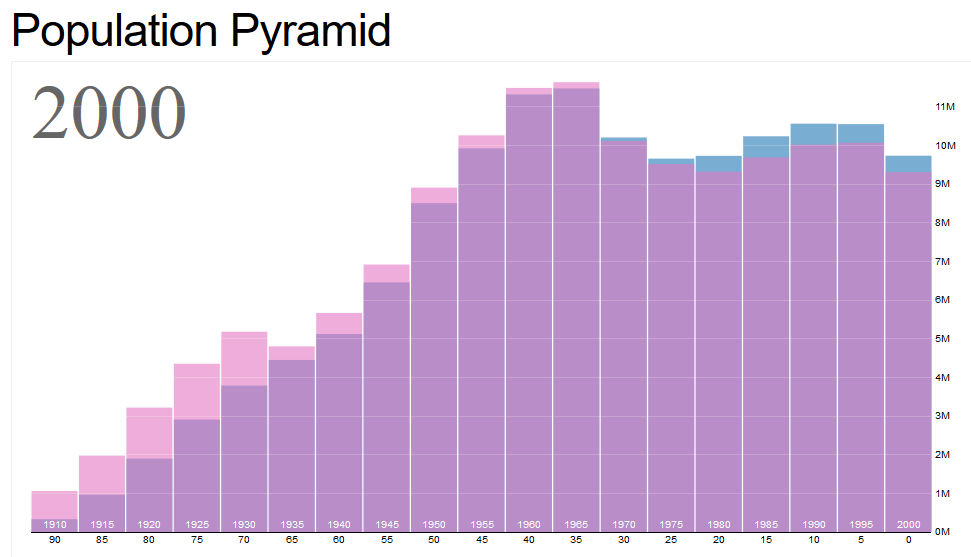
\includegraphics[width=.8\linewidth]{../screenshots/population_d3.PNG}
	\caption{Darstellung einer Alterspyramide mit D3}
	\label{abb:pyramid}
\end{figure}
\begin{figure}
	\centering
	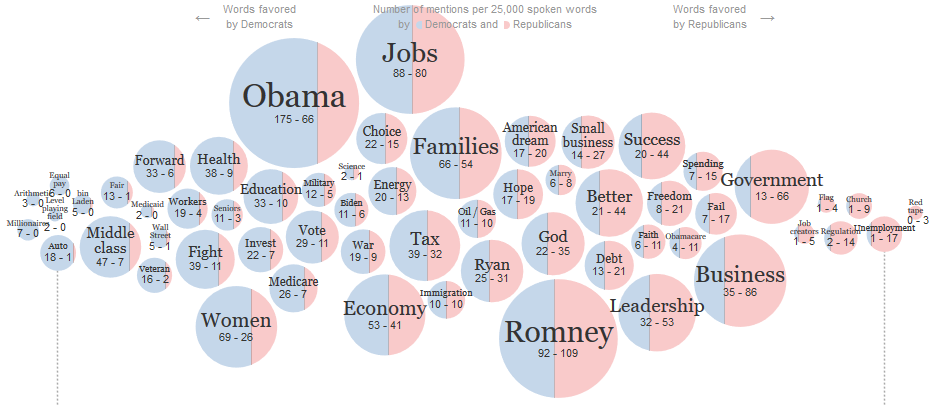
\includegraphics[width=.8\linewidth]{../screenshots/ny_times_d3.PNG}
	\caption{Benutzte Worte bei \glqq National Conventions\grqq\ 2012 in den USA}
	\label{abb:nytimes}
\end{figure}
\subsection{Anwendungsbeispiele}\label{sec:anwendung}
Ein Vorteil von D3 besteht in seiner Verbreitung, die sich in der Menge verschiedenster Anwendungsbeispiele zeigt, welche im Internet zu finden sind. Auf Abbildung \ref{abb:pyramid} sieht man eine Alterspyramide der US-Amerikanischen Bevölkerung im Jahr 2000. \todo{quelle} Daten zu Männern und Frauen sind dabei nicht - wie normalerweise üblich - getrennt voneinander dargestellt, sondern übereinander gelegt. Rosafarbene Balken stehen für Frauen, blaue für Männer und lila zeigt eine Überschneidung beider Farben an. Die x-Achse beschreibt das Alter der Personen und die y-Achse die Bevölkerungszahl. Mit Hilfe der Pfeiltasten kann die Jahreszahl schrittweise bis 1850 zurückgestellt werden, wobei die angezeigten Daten sich immer auf das eingestellte Jahr aktualisieren.

Ein anderes Beispiel, bei dem D3 zum Einsatz kommt, ist in Abbildung \ref{abb:nytimes} zu sehen, die einem Onlineartikel der New York Times entnommen ist. \todo{quelle} Auf den \glqq National Conventions\grqq, welche in den USA traditionell von beiden Parteien vor den Präsidentschaftswahlen abgehalten werden, wurden die gesprochenen Wörter der Redner gezählt und in einem sogenannten Blasendiagramm dargestellt. Je häufiger ein Wort verwendet wurde, desto größer ist dessen Blase. Die Farbaufteilung in rot und blau beschreibt, wie häufig Republikaner bzw. Demokraten das Wort benutzten. Vorwiegend von Republikanern ausgesprochene Wörter finden sich eher auf der rechten Seite wieder, mehrheitlich von Demokraten verwendete Begriffe auf der linken.

Die Verschiedenheit dieser Beispiele macht die Vielseitigkeit von D3 deutlich, welche ein wichtiger Grund für dessen Verbreitung ist.
\subsection{Module}
Da D3 sehr umfangreich ist und die Meisten Anwendungen nicht alle Funktionen benötigen, ist es in Module unterteilt, die einzeln eingebunden werden können. Die für diese Arbeit besonders relevanten Module sind $Selections$, $Hierarchies$, $Shapes$ und $Transitions$.

\subsubsection*{Selections}\label{sec:selections}
$Selections$ sind einer der wichtigsten Bestandteile von D3. Sie dienen dazu, HTML-Elemente zu gruppieren, manipulieren und mit Daten zu verknüpfen. Man erstellt sie mit den Befehlen $d3.select$ oder $d3.selectAll$, wobei $select$ das erste auf die Übergabe passende und $selectAll$ alle passenden Elemente in eine $selection$ zusammenführt.  

Über die Funktion $selection.data$ können die Elemente einer $selection$ mit beliebigen Daten verknüpft werden. Gibt man dabei jedem einzelnen Datensatz eine eindeutige $id$ so teilt D3 automatisch Datensätze und HTML-Elemente in drei Gruppen auf: 
\begin{enumerate}
	\item Daten-Element-Paare, die bereits zuvor verknüpft wurden ($update\ selection$)
	\item Daten, für die noch kein HTML-Objekt existiert ($enter\ selection$)
	\item HTML-Elemente, für die kein Datensatz vorhanden ist ($exit\ selection$).
\end{enumerate}

In vielen Fällen, wie zum Beispiel durch Nutzereingaben bei der in Kapitel \ref{sec:anwendung} beschriebenen Alterspyramide, kann es zu Änderungen der Daten kommen, die bereits Auf dem Bildschirm zu sehen sind. In solchen Fällen kommt die $update\ selection$ zum Einsatz. Sie ist die $selection$, die beim Aufruf von $selection.data$ zurückgegeben wird und dient - wie der Name sagt - zur Aktualisierung der angezeigten Objekte. Beispielsweise können mit der Funktion $selection.attr$ HTML-Attribute angepasst oder mit $selection.class$ CSS-Klassen gesetzt werden. Jede auf einer $selection$ aufgerufene Funktion wird dabei auf alle in ihr enthaltenen Objekte einzeln angewendet. Über die $update\ selection$ hat man außerdem Zugriff auf die $enter$ und $exit\ selection$.

Die $enter\ selection$ erhält man durch den Funktionsaufruf $selection.enter$. Um HTML-Objekte für diese bisher nicht visualisierten Informationen hinzuzufügen wendet man die Methode $selection.append$ auf die $enter\ selection$ an und benennt dabei das anzuhängende Element. $Append$ erstellt dann für jeden der Datensätze in der $selection$ ein HTML-Element dieser Art und verknüpft die beiden miteinander.

Meist gilt für Objekte in der $exit\ selection$, dass sie nicht mehr angezeigt werden sollen, weil es keine korrespondierenden Daten mehr gibt. In diesem Fall kann mit einem Aufruf von $selection.exit$ auf sie zugegriffen und alle Elemente durch $selection.remove$ entfernt werden.

\subsubsection*{Hierarchies}\label{sec:hierarchies}
Mit Hilfe von D3 $hierarchies$ können Daten verarbeitet werden, die hierarchisch angeordnet sind, wie zum Beispiel Familienstammbäume oder Dateisysteme. Einzelne Datenpunkte werden dabei auch als Knoten ($node$) bezeichnet. Die Daten unterliegen den gleichen Regeln, wie die Knoten eines Baumes (Kapitel \ref{sec:baum}), das heißt es gibt genau eine Wurzel und alle anderen Knoten haben einen Vorgänger und beliebig viele Nachfolger. Aufgrund dieser Eigenschaften kann eine $hierarchy$ als Baum visualisiert werden. Die Funktion $d3.hierarchy$ nimmt ein Javascript-Objekt entgegen, dass die Wurzel repräsentiert und erzeugt daraus eine $hierarchy$, in der jeder Knoten seine ursprünglichen Daten enthält und zusätzlich diverse Hilfsfunktionen, wie $node.descendants$, die eine Liste aller Nachfolgenden Knoten zurückgibt, oder $node.path$ zur Berechnung des kürzesten Pfades zum übergebenen Zielknoten.

Die Funktion $d3.tree$ berechnet unter Verwendung des Reingold-Tilford-Algorithmus (\citet{reingold1981tidier}) eine Knotenanordnung für die Darstellung einer $hierarchy$ als Baum. Dadurch erhält jeder Knoten eine x- und y-Koordinate im Bereich von 0 bis 1, die bei der Visualisierung beliebig skaliert werden können.

\subsubsection*{Shapes}
Das $shapes$ Modul dient zur Darstellung von beliebigen Formen. Es liefert dabei für verschiedene Anwendungsfälle unterstützende Funktionen. Es wird bei der hier beschriebenen Visualisierung von Bäumen verwendet, um die Kanten in Form von Linien zu zeichnen und für die Berechnung des Eingabemenüs (Kapitel \ref{sec:kanten} und \ref{sec:eingabemenu}). Dabei kommen insbesondere die Funktionen $d3.line$, $d3.pie$ und $d3.arc$ zum Einsatz.

$D3.line$ generiert aus einem Start- und Endpunkt-Paar eine Reihe von Anweisungen zum Zeichnen einer Linie, die an ein $path$-Element in einem $svg$ übergeben werden kann. 
\begin{figure}
	\centering
	\begin{minipage}{.5\textwidth}
	\centering
	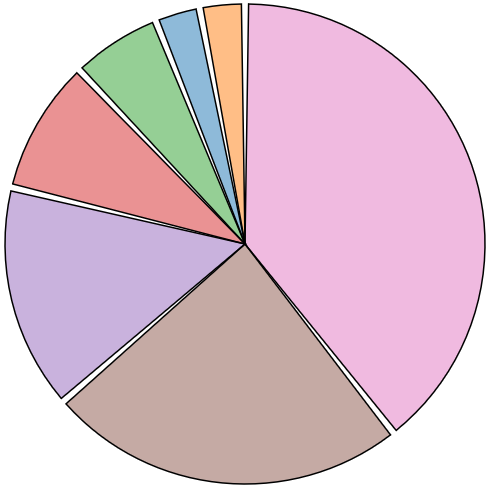
\includegraphics[width=.8\linewidth]{../screenshots/kreisdiagramm.PNG}
	\caption{Ein Kreisdiagramm}
	\label{abb:kreisdiagramm}
	\end{minipage}%
	\begin{minipage}{.5\textwidth}
	\centering
	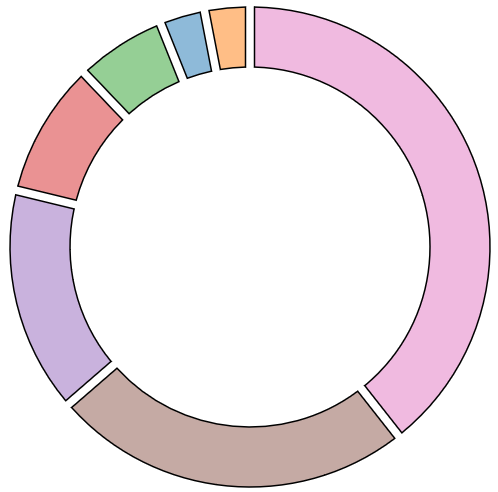
\includegraphics[width=.8\linewidth]{../screenshots/donutchart.PNG}
	\caption{Ein Ringdiagramm}
	\label{abb:donut}
	\end{minipage}
\end{figure}
$D3.arc$ und $d3.pie$ können zusammen benutzt werden, um Ringdiagramme zu erzeugen. Abbildung \ref{abb:donut} zeigt ein so mit D3 erzeugtes Ringdiagramm \todo{quelle} bestehend aus sieben Segmenten. $D3.arc$ wird verwendet um einen Bogengenerator zu erzeugen, der zu Übergaben von Start- und Endwinkeln passende Kreisbögen generiert. $D3.pie$ erstellt aus einer Liste von Daten, wie zum Beispiel Stimmenanteilen bei einer Wahl, die nötigen Übergaben, damit der Bogengenerator automatisch ein passendes Ringdiagramm erzeugt. Man kann dabei unter Einsatz der Funktionen $arc.innerRadius$ und $arc.outerRadius$ den Innen- und Außenradius des erzeugten Rings festlegen, wobei ein Innenradius von 0 zur Erzeugung eines Kreisdiagramms führt (Abbildung \ref{abb:kreisdiagramm}).

\subsubsection*{Transitions}
\begin{figure}
	\centering
	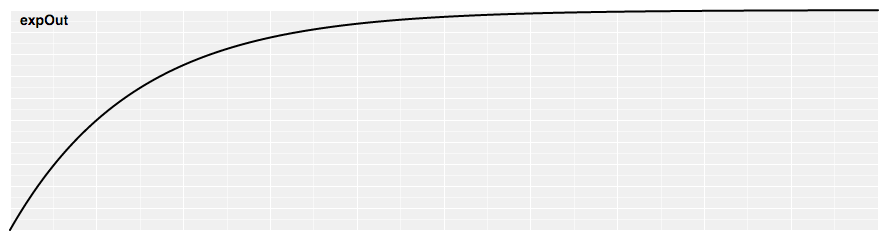
\includegraphics[width=\linewidth]{../screenshots/expOut.png}
	\caption{Die Übergangsfunktion $easeExpOut$}
	\label{abb:easing}
\end{figure}
$Transitions$ bauen auf dem Konzept von $selections$ auf und dienen dazu, Veränderungen an Angezeigten Objekten nicht abrupt vorzunehmen, sondern in gleichmäßigen Abstufungen vom Startzustand zum Endzustand überzugehen. Auf diese Weise können vielfältige Animationen realisiert werden. Man startet eine $transition$ durch den Aufruf von $selection.transition$ und kann anschließend alle Anzeigeänderungen, die man an der $selection$ vornehmen kann auch über die zurückgegebene $transition$ erreichen. Dabei kann mit der Funktion $transition.duration$ eine Dauer und mit $transition.delay$ eine Verzögerung des Übergangs in Millisekunden angegeben werden. Darüber hinaus bietet $transition.ease$ die Möglichkeit eine Übergangsfunktion zu bestimmen, die vorgibt wie schnell sich der jeweilige Wert zu gegebenen Zeitpunkten ändert. Zum Beispiel kann eine Bewegung schnell beginnen und zum Ende hin langsamer werden, wofür die Übergangsfunktion $easeExpOut$ geeignet wäre, deren Funktionsgraph in Abbildung \ref{abb:easing} \todo{quelle} zu sehen ist. D3 bringt bereits eine Reihe solcher Funktionen mit, es können aber auch eigene definiert werden.

\section{Struktur der verwendeten Daten}\label{sec:inputdaten}
\todo{aufzählen, welche eigenschaften die übergebenen knoten haben. diagnosis, etc.}
































